\documentclass{standalone}
\usepackage{tikz}
\usepackage{pgfplots}
\usepackage{pgfplotstable}
\usetikzlibrary{plotmarks, calc}
\pgfplotsset{compat=1.13}
\begin{document}
  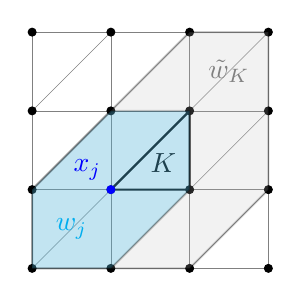
\begin{tikzpicture}
    % Square grid
    \draw[step=1cm, gray, very thin] (0, 0) grid (3, 3);
    % Triangles
    \foreach \x in {0, 1, 2}{
      \foreach \y in {0, 1, 2}{
        \draw[gray, very thin] (\x, \y) -- (\x+1, \y+1);
      }
    }
    % Vertices
    \foreach \x in {0, 1, 2, 3}{
      \foreach \y in {0, 1, 2, 3}{
         \node[draw, circle, inner sep=1pt, fill] at (\x, \y) { };
      }
    }
    % The interpolated element K
    \draw [thick, draw=black]%, fill=yellow, opacity=0.2]
    (1, 1) -- (2, 1) -- (2, 2) -- cycle;
    \node at (5/3., 4/3.) {$K$};
    % Patch which controls the error
    \draw [thick, draw=black, fill=lightgray, opacity=0.2]
    (0, 0)--(2, 0)--(3, 1)--(3, 3)--(2, 3)--(0, 1)--(0, 0);
    \node[gray] at (5/2., 5/2.) {$\tilde{w}_K$};
    % Patch of w_j
    \draw [thick, draw=black, fill=cyan, opacity=0.2]
    (0, 0)--(1, 0)--(2, 1)--(2, 2)--(1, 2)--(0, 1)--(0, 0);
    \node[cyan] at (1/2., 1/2.) {$w_j$};
    % The vertex xj
    \node[blue, draw, circle, inner sep=1pt, fill] at (1, 1) { };
    \node[blue, above left] at (1, 1) {$x_j$};
  \end{tikzpicture}
\end{document}
